%###############################################################################
%# N1 - Manual - Architecture Description                                      #
%###############################################################################
%#    Copyright 2018 - 2022 Dirk Heisswolf                                     #
%#    This file is part of the N1 project.                                     #
%#                                                                             #
%#    N1 is free software: you can redistribute it and/or modify               #
%#    it under the terms of the GNU General Public License as published by     #
%#    the Free Software Foundation, either version 3 of the License, or        #
%#    (at your option) any later version.                                      #
%#                                                                             #
%#    N1 is distributed in the hope that it will be useful,                    #
%#    but WITHOUT ANY WARRANTY; without even the implied warranty of           #
%#    MERCHANTABILITY or FITNESS FOR A PARTICULAR PURPOSE.  See the            #
%#    GNU General Public License for more details.                             #
%#                                                                             #
%#    You should have received a copy of the GNU General Public License        #
%#    along with N1.  If not, see <http://www.gnu.org/licenses/>.              #
%###############################################################################
%# Version History:                                                            #
%#   November 11, 2022                                                         #
%#      - Initial release                                                      #
%###############################################################################

\section{Architecture Description}
\label{architecture}

The following sections provide some descriptions of the internal N1 design.


\subsection{Design Principles}
\label{architecture:principles}

The RTL implementation of the N1 follows a number of design principles which are captured in following sections. 

\subsubsection{Naming Convention of Interface Signals}
\label{architecture:principles:naming}

For all signals, which do not implement a common standard (e.g. \gls{wb}),
the following signal naming rules are used throughout the design:
\begin{itemize}

\item
Signals which are grouped into an interface are prefixed with a meaningful interface name.\\
Example: \texttt{\underline{ups\_}push}

  
\item
All other point-to-point connections, contain a mnemonic of the sending and the receiving block in its prefix.
The format of the prefix is: \\
\emph{\textless sender mnemonic\textgreater}\texttt{2}\emph{\textless receiver mnemonic\textgreater }\texttt{\_}\dots \\
Example: \texttt{\underline{fc2ir\_}capture}

\item   
Control signals which represent a request, end with a verb in imperative form. \\
Example: \texttt{fc2ir\_\underline{expend}}

\item   
Status signals represening a busy indicator, have the postfix \dots\texttt{\_bsy} \\
Example: \texttt{prs2fc\_\underline{bsy}}

\item   
If a signal is connected to the interface of a module, a further postfix is added to indicate the signal direction:
  \begin{itemize}
    \item   
    Input signals: \dots\texttt{\_i} \\
    \item   
    Output signals: \dots\texttt{\_o} \\
  \end{itemize}
Example: \texttt{prs2fc\_bsy\underline{\_o}}
  
\item   
Names of signals which are only used within one design block are kept short and don't follow a particular naming convention.

\end{itemize}

\subsubsection{Handshaking}
\label{architecture:principles:handshakes}

A high signal level of a contol signal is interpreted a request by the receiving design block.
The request is expected to be immediately accepted by the receiver and processed in the next clock cycle,
unless the receiver provides a busy indicator (\dots\texttt{\_bsy}).
In this case the request in only accepted if the busy indicator was deasserted in the cycle, in which the request is made.

\subsection{Common Internal Interfaces}
\label{architecture:interfaces}

The subblocks in the N1 design use common interfaces for common functionality. These interfaces follow the
\hyperref[architecture:principles:naming]{naming conventions} and \hyperref[architecture:principles:handshakes]{handshaking concept} 
described in \secref{architecture:principles}.

\subsubsection{Stack Interface}
\label{architecture:interfaces:stack}

All stacks are controlled using the following interface:
\begin{description}[style=nextline]

\item[\emph{\textless stack name\textgreater}\texttt{\_clear\_o}/\texttt{\_i} {\scriptsize (controller $\rightarrow$ stack)}]
  Request to clear the stack.
  
\item[\emph{\textless stack name\textgreater}\texttt{\_clear\_bsy\_i}/\texttt{\_o} {\scriptsize (controller $\leftarrow$ stack)}]
  Busy indicator. \\
  The stack will be cleared if \emph{\textless stack name\textgreater}\texttt{\_clear\_i} is asseeted while \\
  \emph{\textless stack name\textgreater}\texttt{\_clear\_bsy\_o} is deasserted.

\item[\emph{\textless stack name\textgreater}\texttt{\_push\_o}/\texttt{\_i} {\scriptsize (controller $\rightarrow$ stack)}]
  Request to push a data word onto the stack.

\item[\emph{\textless stack name\textgreater}\texttt{\_push\_data\_o}/\texttt{\_i[15:0]} {\scriptsize (controller $\rightarrow$ stack)}]
  Data word to be pushed onto the stack. \\
  The data word must be supplied in the same clock cycle as the request.

\item[\emph{\textless stack name\textgreater}\texttt{\_push\_bsy\_i}/\texttt{\_o} {\scriptsize (controller $\leftarrow$ stack)}]
  Busy indicator. \\
  \emph{\textless stack name\textgreater}\texttt{\_push\_data\_i} will be pushed onto the stack if
  \emph{\textless stack name\textgreater}\texttt{\_push\_i} is asserted while
  \emph{\textless stack name\textgreater}\texttt{\_push\_bsy\_o} and 
  \emph{\textless stack name\textgreater}\texttt{\_full\_o} are deasserted.
  
\item[\emph{\textless stack name\textgreater}\texttt{\_full\_i}/\texttt{\_o} {\scriptsize (controller $\leftarrow$ stack)}]
  Overflow indicator. \\
  \emph{\textless stack name\textgreater}\texttt{\_full\_o} is asserted when the stack is full and a new push request would cause an overflow.

\item[\emph{\textless stack name\textgreater}\texttt{\_pull\_o}/\texttt{\_i} {\scriptsize (controller $\rightarrow$ stack)}]
  Request to pull a data word from the stack.

\item[\emph{\textless stack name\textgreater}\texttt{\_pull\_data\_i}/\texttt{\_o[15:0]} {\scriptsize (controller $\leftarrow$ stack)}]
  Data word to be pulled from the stack. If the stack is not empty \\
  (\emph{\textless stack name\textgreater}\texttt{\_empty\_o} deasserted)
  and ready for a pull operation \\
  (\emph{\textless stack name\textgreater}\texttt{\_pull\_bsy\_o} deasserted),
  then \emph{\textless stack name\textgreater}\texttt{\_pull\_data\_o} always shows the data at the top of the stack.

\item[\emph{\textless stack name\textgreater}\texttt{\_pull\_bsy\_i}/\texttt{\_o} {\scriptsize (controller $\leftarrow$ stack)}]
  Busy indicator. \\
  The data at the top of the stack will be removed if
  \emph{\textless stack name\textgreater}\texttt{\_pull\_i} is asserted while
  \emph{\textless stack name\textgreater}\texttt{\_pull\_bsy\_o} and 
  \emph{\textless stack name\textgreater}\texttt{\_empty\_o} are deasserted.

\item[\emph{\textless stack name\textgreater}\texttt{\_empty\_i}/\texttt{\_o} {\scriptsize (controller $\leftarrow$ stack)}]
  Underflow indicator. \\
  \emph{\textless stack name\textgreater}\texttt{\_empty\_o} is asserted when the stack is empty and a new pull request would cause an underflow.

\end{description}

The stack interface is also used for FIFOs.

\subsubsection{Memory Interface}
\label{architecture:interfaces:memory}

Memories are connected through the following interface:
\begin{description}[style=nextline]

\item[\emph{\textless memory name\textgreater}\texttt{\_addr\_o}/\texttt{\_i[$n$-1:0]} {\scriptsize (controller $\rightarrow$ memory)}]
  Memory address.

\item[\emph{\textless memory name\textgreater}\texttt{\_access\_o}/\texttt{\_i} {\scriptsize (controller $\rightarrow$ memory)}]
  Access request.
  
\item[\emph{\textless memory name\textgreater}\texttt{\_rwb\_o}/\texttt{\_i} {\scriptsize (controller $\rightarrow$ memory)}]
  Data direction selector (high for read, low fro write).
  
\item[\emph{\textless memory name\textgreater}\texttt{\_access\_bsy\_i}/\texttt{\_o} {\scriptsize (controller $\leftarrow$ memory)}]
  Busy indicator. \\
  A request is valid if
  \emph{\textless memory name\textgreater}\texttt{\_access\_i} is asserted while \\
  \emph{\textless memory name\textgreater}\texttt{\_access\_bsy\_o} is deasserted.
  
\item[\emph{\textless memory name\textgreater}\texttt{\_wdata\_o}/\texttt{\_i[15:0]} {\scriptsize (controller $\rightarrow$ memory)}]
  Write data. \\
  Write data must be driven in the same clock cycle as the request.
  
\item[\emph{\textless memory name\textgreater}\texttt{\_rdata\_i}/\texttt{\_o[15:0]} {\scriptsize (controller $\leftarrow$ memory)}]
  Read data. \\
  Read data must be captured one clock cyle after a valid request has been captured, unless a delay is indicated. 

\item[\emph{\textless memory name\textgreater}\texttt{\_rdata\_del\_o}/\texttt{\_i[15:0]} {\scriptsize (controller $\rightarrow$ memory)}]
  Read data delay indicator. \\
  If asserted, this signalwill postpone expected read data by one clock cycle..

\end{description}

\subsubsection{Register Interface}
\label{architecture:interfaces:registers}

Registers are accessed through the following interface:
\begin{description}[style=nextline]

\item[\emph{\textless register block name\textgreater}\texttt{\_addr\_o}/\texttt{\_i[$n$-1:0]} {\scriptsize (controller $\rightarrow$ register block)}]
  Register address.

\item[\emph{\textless register block name\textgreater}\texttt{\_set\_o}/\texttt{\_i} {\scriptsize (controller $\rightarrow$ register block)}]
  Register write request. \\
  Register address and write data must be supplied in the same clock cycle as the write request.
  
\item[\emph{\textless register block name\textgreater}\texttt{\_set\_data\_o}/\texttt{\_i[$n$-1:0]} {\scriptsize (controller $\rightarrow$ register block)}]
  Register write data.

\item[\emph{\textless register block name\textgreater}\texttt{\_set\_bsy\_i}/\texttt{\_o} {\scriptsize (controller $\leftarrow$ register block)}]
  Register write busy indicator.

\item[\emph{\textless register block name\textgreater}\texttt{\_get\_o}/\texttt{\_i} {\scriptsize (controller $\rightarrow$ register block)}]
  Register read request.\\
  The register address must be supplied in the same clock cycle as the write request. Unless the busy indicator is asserted, read data is available in
  the same clock cycle as the request.

\item[\emph{\textless register block name\textgreater}\texttt{\_get\_data\_o}/\texttt{\_i[$n$-1:0]} {\scriptsize (controller $\rightarrow$ register block)}]
  Register read data.

\item[\emph{\textless register block name\textgreater}\texttt{\_get\_bsy\_i}/\texttt{\_o} {\scriptsize (controller $\leftarrow$ register block)}]
  Register read busy indicator.

\end{description}

\subsubsection{Instruction Boundaries}
\label{architecture:principles:ibounds}

The \hyperref[architecture:comp:ir]{instruction register} always contains the instruction which is currently in execution.
Before the execution of an instruction can ce concluded and the next one can begin, the fillowing conditions must be fulfilled:
\begin{itemize}

\item   
The program bus must be available - TBD
  
\item   
The parameter and the return stack must be available - TBD
  
\end{itemize}

\subsection{Instruction Execution Cycle}
\label{architecture:excyc}

The execution cycle of the N1 processor characterized by the following design components:
\begin{description}[style=nextline]

\item[\textbf{Program Counter}]
A 16-bit register, which contains the memory location on the next instruction to be executed.  
It is implemented within the \hyperref[architecture:comp:dsp]{DSP Block}.

\item[\textbf{Address Bus}]
The address output of the \hyperref[integration:if:pbus]{Program Bus (\texttt{pbus\_adr\_o})}.

\item[\textbf{Read Data Bus}]
The read data input of the \hyperref[integration:if:pbus]{Program Bus (\texttt{pbus\_dat\_i})}

\item[\textbf{Instruction Register}]
A 16-bit register holding the opcode of the instruction, which is currently executed (see \secref{architecture:comp:ir}).

\item[\textbf{Instruction Stash Register}]
A 16-bit register to temoprarily store an upcoming opcode. (see \secref{architecture:comp:ir}).

\end{description}

The following sections show the timing relation of these design components in different execution scenarios.


\subsubsection{Plain Linear Execution}
\label{architecture:excyc:linear}

Most of of the  N1 instructuins are executed in a single clock cycle.
\figref{architecture:excyc:linear:fig} the typical linear execution flow of single cycle instructions.

The opcode stored in the instruction register determines which instruction is currently being executed.
The program counter points to the address of the next instruction.
The address bus is unregistered and always runs one clock cycle ahead of the program counter. 
The resulting data on the read data bus is captured by the instruction register in the next clock cycle.

    
\begin{figure}[!h]
  \begin{center}
  \makebox[\textwidth][c]{
  \scalebox{1} {
      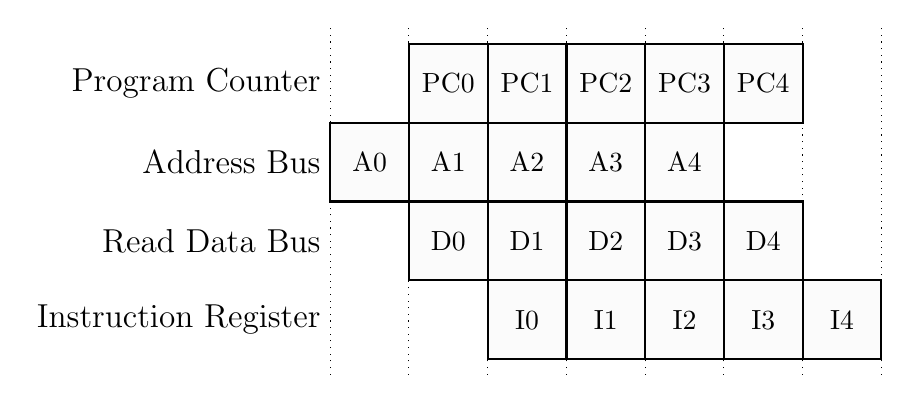
\begin{tikzpicture}

        %Lines
        \draw [dotted] (0,0.3) -- (0,4.7);
        \draw [dotted] (1,0.3) -- (1,4.7);
        \draw [dotted] (2,0.3) -- (2,4.7);
        \draw [dotted] (3,0.3) -- (3,4.7);
        \draw [dotted] (4,0.3) -- (4,4.7);
        \draw [dotted] (5,0.3) -- (5,4.7);
        \draw [dotted] (6,0.3) -- (6,4.7);
        \draw [dotted] (7,0.3) -- (7,4.7);

        %Program counter
        \node  [left] at (0,4) {\large{Program Counter}};
        \draw [thick, fill=gray!3] (1,4.5) rectangle (2,3.5);
        \node at (1.5,4)  {PC0};
        \draw [thick, fill=gray!3] (2,4.5) rectangle (3,3.5);
        \node at (2.5,4)  {PC1};
        \draw [thick, fill=gray!3] (3,4.5) rectangle (4,3.5);
        \node at (3.5,4)  {PC2};
        \draw [thick, fill=gray!3] (4,4.5) rectangle (5,3.5);
        \node at (4.5,4)  {PC3};
        \draw [thick, fill=gray!3] (5,4.5) rectangle (6,3.5);
        \node at (5.5,4)  {PC4};
        
        %Address bus
        \node [left] at (0,3) {\large{Address Bus}};
        \draw [thick, fill=gray!3] (0,3.5) rectangle (1,2.5);
        \node at (0.5,3)  {A0};
        \draw [thick, fill=gray!3] (1,3.5) rectangle (2,2.5);
        \node at (1.5,3)  {A1};
        \draw [thick, fill=gray!3] (2,3.5) rectangle (3,2.5);
        \node at (2.5,3)  {A2};
        \draw [thick, fill=gray!3] (3,3.5) rectangle (4,2.5);
        \node at (3.5,3)  {A3};
        \draw [thick, fill=gray!3] (4,3.5) rectangle (5,2.5);
        \node at (4.5,3)  {A4};

        %Read data bus
        \node [left] at (0,2) {\large{Read Data Bus}};
        \draw [thick, fill=gray!3] (1,2.5) rectangle (2,1.5);
        \node at (1.5,2)  {D0};
        \draw [thick, fill=gray!3] (2,2.5) rectangle (3,1.5);
        \node at (2.5,2)  {D1};
        \draw [thick, fill=gray!3] (3,2.5) rectangle (4,1.5);
        \node at (3.5,2)  {D2};
        \draw [thick, fill=gray!3] (4,2.5) rectangle (5,1.5);
        \node at (4.5,2)  {D3};
        \draw [thick, fill=gray!3] (5,2.5) rectangle (6,1.5);
        \node at (5.5,2)  {D4};

        %Instruction register
        \node [left] at (0,1) {\large{Instruction Register}};
        \draw [thick, fill=gray!3] (2,1.5) rectangle (3,0.5);
        \node at (2.5,1)  {I0};
        \draw [thick, fill=gray!3] (3,1.5) rectangle (4,0.5);
        \node at (3.5,1)  {I1};
        \draw [thick, fill=gray!3] (4,1.5) rectangle (5,0.5);
        \node at (4.5,1)  {I2};
        \draw [thick, fill=gray!3] (5,1.5) rectangle (6,0.5);
        \node at (5.5,1)  {I3};
        \draw [thick, fill=gray!3] (6,1.5) rectangle (7,0.5);
        \node at (6.5,1)  {I4};

      \end{tikzpicture}
    }
  }
  \caption{Plain Linear Execution}
  \label{architecture:excyc:linear:fig}
  \end{center}
\end{figure}


\subsubsection{Execution of Extended Instructions}
\label{architecture:excyc:extended}

In some cases the execution of an instruction can span multiple cycles (i.e. \hyperref[opcodes:ctrl]{non-concurrent control instructions}
or any instruction waiting for a blocked stack access). 
\figref{architecture:excyc:extended:fig} illustrates the timing in these scenarios.

Whenever an opcode needs to be captured from the read data bus, but the instruction register is blocked by an instruction spaning multiple cycles,
The incoming opcode needs to be temourarely stashed away in a separate register.
When the execution of the ongoing instruction is finished, the stashed opcode is moved into the instruction register.

\begin{figure}[!h]
  \begin{center}
  \makebox[\textwidth][c]{
  \scalebox{1} {
      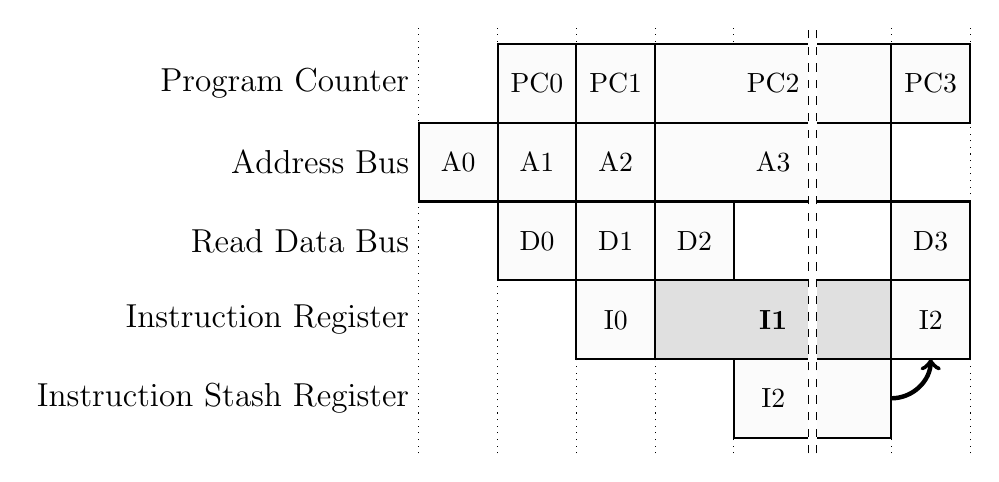
\begin{tikzpicture}

        %Lines
        \draw [dotted] (0,-0.7) -- (0,4.7);
        \draw [dotted] (1,-0.7) -- (1,4.7);
        \draw [dotted] (2,-0.7) -- (2,4.7);
        \draw [dotted] (3,-0.7) -- (3,4.7);
        \draw [dotted] (4,-0.7) -- (4,4.7);
        %\draw [dotted] (5,-0.7) -- (5,4.7);
        \draw [dotted] (6,-0.7) -- (6,4.7);
        \draw [dotted] (7,-0.7) -- (7,4.7);

        %Program counter
        \node  [left] at (0,4) {\large{Program Counter}};
        \draw [thick, fill=gray!3] (1,4.5) rectangle (2,3.5);
        \node at (1.5,4)  {PC0};
        \draw [thick, fill=gray!3] (2,4.5) rectangle (3,3.5);
        \node at (2.5,4)  {PC1};
        \draw [thick, fill=gray!3] (3,4.5) rectangle (6,3.5);
        \node  at (4.5,4)  {PC2};
        \draw [thick, fill=gray!3] (6,4.5) rectangle (7,3.5);
        \node at (6.5,4)  {PC3};
        
        %Address bus
        \node [left] at (0,3) {\large{Address Bus}};
        \draw [thick, fill=gray!3] (0,3.5) rectangle (1,2.5);
        \node at (0.5,3)  {A0};
        \draw [thick, fill=gray!3] (1,3.5) rectangle (2,2.5);
        \node at (1.5,3)  {A1};
        \draw [thick, fill=gray!3] (2,3.5) rectangle (3,2.5);
        \node at (2.5,3)  {A2};
        \draw [thick, fill=gray!3] (3,3.5) rectangle (6,2.5);
        \node at (4.5,3)  {A3};

        %Read data bus
        \node [left] at (0,2) {\large{Read Data Bus}};
        \draw [thick, fill=gray!3] (1,2.5) rectangle (2,1.5);
        \node at (1.5,2)  {D0};
        \draw [thick, fill=gray!3] (2,2.5) rectangle (3,1.5);
        \node at (2.5,2)  {D1};
        \draw [thick, fill=gray!3] (3,2.5) rectangle (4,1.5);
        \node at (3.5,2)  {D2};
        \draw [thick, fill=gray!3] (6,2.5) rectangle (7,1.5);
        \node at (6.5,2)  {D3};

        %Instruction register
        \node [left] at (0,1) {\large{Instruction Register}};
        \draw [thick, fill=gray!3] (2,1.5) rectangle (3,0.5);
        \node at (2.5,1)  {I0};
        \draw [thick, fill=gray!24] (3,1.5) rectangle (6,0.5);
        \node at (4.5,1)  {\textbf{I1}};
        \draw [thick, fill=gray!3] (6,1.5) rectangle (7,0.5);
        \node at (6.5,1)  {I2};

        %Instruction stashregister
        \node [left] at (0,0) {\large{Instruction Stash Register}};
        \draw [thick, fill=gray!3] (4,0.5) rectangle (6,-0.5);
        \node at (4.5,0)  {I2};
        %\draw [ultra thick, ->]  (5,0) -- (5.5,0) -- (5.5,0.5);
        \draw [ultra thick, ->] (6,0) arc (270:360:0.5) ;

        %Gap
        %\draw [dotted] (5,-0.7) -- (5,4.7);
        \draw [fill=white, white] (4.95,-0.7) rectangle (5.05,4.7);
        \draw [dashed] (4.95,-0.7) -- (4.95,4.7);
        \draw [dashed] (5.05,-0.7) -- (5.05,4.7);

        
      \end{tikzpicture}
    }
  }
  \caption{Execution of an Extended Instruction}
  \label{architecture:excyc:extended:fig}
  \end{center}
\end{figure}


\subsubsection{Execution of Memory Access Instructions}
\label{architecture:excyc:mem}

A special case of multi-cycle instructions are \hyperref[opcodes:memacc]{memory access instructions}.
These instructions perform their memory acesses on the program bus.
\figref{architecture:excyc:mem:fig} illustrates how opcode fetches and data accesses are interleaved.

\begin{figure}[!h]
  \begin{center}
  \makebox[\textwidth][c]{
  \scalebox{1} {
      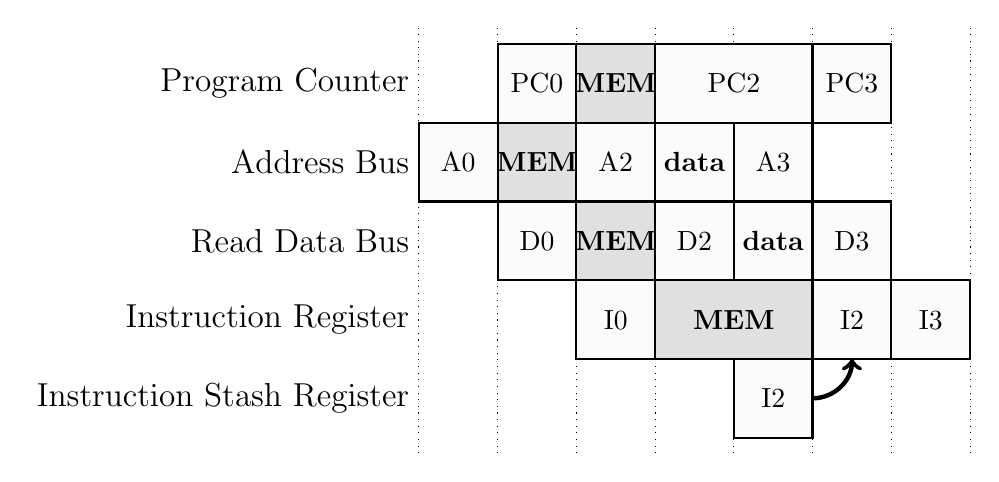
\begin{tikzpicture}

        %Lines
        \draw [dotted] (0,-0.7) -- (0,4.7);
        \draw [dotted] (1,-0.7) -- (1,4.7);
        \draw [dotted] (2,-0.7) -- (2,4.7);
        \draw [dotted] (3,-0.7) -- (3,4.7);
        \draw [dotted] (4,-0.7) -- (4,4.7);
        \draw [dotted] (5,-0.7) -- (5,4.7);
        \draw [dotted] (6,-0.7) -- (6,4.7);
        \draw [dotted] (7,-0.7) -- (7,4.7);

        %Program counter
        \node  [left] at (0,4) {\large{Program Counter}};
        \draw [thick, fill=gray!3] (1,4.5) rectangle (2,3.5);
        \node at (1.5,4)  {PC0};
        \draw [thick, fill=gray!24] (2,4.5) rectangle (3,3.5);
        \node at (2.5,4)  {\textbf{MEM}};
        \draw [thick, fill=gray!3] (3,4.5) rectangle (5,3.5);
        \node  at (4,4)  {PC2};
        \draw [thick, fill=gray!3] (5,4.5) rectangle (6,3.5);
        \node at (5.5,4)  {PC3};
        
        %Address bus
        \node [left] at (0,3) {\large{Address Bus}};
        \draw [thick, fill=gray!3] (0,3.5) rectangle (1,2.5);
        \node at (0.5,3)  {A0};
        \draw [thick, fill=gray!24] (1,3.5) rectangle (2,2.5);
        \node at (1.5,3)  {\textbf{MEM}};
        \draw [thick, fill=gray!3] (2,3.5) rectangle (3,2.5);
        \node at (2.5,3)  {A2};
        \draw [thick, fill=gray!3] (3,3.5) rectangle (4,2.5);
        \node at (3.5,3)  {\textbf{data}};
        \draw [thick, fill=gray!3] (4,3.5) rectangle (5,2.5);
        \node at (4.5,3)  {A3};

        %Read data bus
        \node [left] at (0,2) {\large{Read Data Bus}};
        \draw [thick, fill=gray!3] (1,2.5) rectangle (2,1.5);
        \node at (1.5,2)  {D0};
        \draw [thick, fill=gray!24] (2,2.5) rectangle (3,1.5);
        \node at (2.5,2)  {\textbf{MEM}};
        \draw [thick, fill=gray!3] (3,2.5) rectangle (4,1.5);
        \node at (3.5,2)  {D2};
        \draw [thick, fill=gray!3] (4,2.5) rectangle (5,1.5);
        \node at (4.5,2)  {\textbf{data}};
        \draw [thick, fill=gray!3] (5,2.5) rectangle (6,1.5);
        \node at (5.5,2)  {D3};

        %Instruction register
        \node [left] at (0,1) {\large{Instruction Register}};
        \draw [thick, fill=gray!3] (2,1.5) rectangle (3,0.5);
        \node at (2.5,1)  {I0};
        \draw [thick, fill=gray!24] (3,1.5) rectangle (5,0.5);
        \node at (4,1)  {\textbf{MEM}};
        \draw [thick, fill=gray!3] (5,1.5) rectangle (6,0.5);
        \node at (5.5,1)  {I2};
        \draw [thick, fill=gray!3] (6,1.5) rectangle (7,0.5);
        \node at (6.5,1)  {I3};

        %Instruction stash register
        \node [left] at (0,0) {\large{Instruction Stash Register}};
        \draw [thick, fill=gray!3] (4,0.5) rectangle (5,-0.5);
        \node at (4.5,0)  {I2};
        %\draw [ultra thick, ->]  (5,0) -- (5.5,0) -- (5.5,0.5);
        \draw [ultra thick, ->] (5,0) arc (270:360:0.5) ;

      \end{tikzpicture}
    }
  }
  \caption{Execution of a Memory Access Instruction}
  \label{architecture:excyc:mem:fig}
  \end{center}
\end{figure}


\subsubsection{Change of Flow Instructions}
\label{architecture:excyc:cof}

%Change of flow instructions
TBD

\begin{figure}[!h]
  \begin{center}
  \makebox[\textwidth][c]{
  \scalebox{1} {
      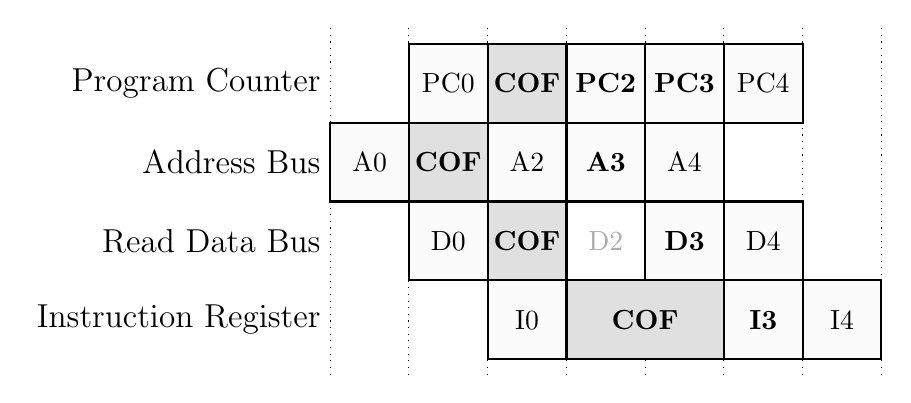
\begin{tikzpicture}

        %Lines
        \draw [dotted] (0,0.3) -- (0,4.7);
        \draw [dotted] (1,0.3) -- (1,4.7);
        \draw [dotted] (2,0.3) -- (2,4.7);
        \draw [dotted] (3,0.3) -- (3,4.7);
        \draw [dotted] (4,0.3) -- (4,4.7);
        \draw [dotted] (5,0.3) -- (5,4.7);
        \draw [dotted] (6,0.3) -- (6,4.7);
        \draw [dotted] (7,0.3) -- (7,4.7);

        %Program counter
        \node  [left] at (0,4) {\large{Program Counter}};
        \draw [thick, fill=gray!3] (1,4.5) rectangle (2,3.5);
        \node at (1.5,4)  {PC0};
        \draw [thick, fill=gray!24] (2,4.5) rectangle (3,3.5);
        \node at (2.5,4)  {\textbf{COF}};
        \draw [thick, fill=gray!3] (3,4.5) rectangle (4,3.5);
        \node at (3.5,4)  {\textbf{PC2}};
        \draw [thick, fill=gray!3] (4,4.5) rectangle (5,3.5);
        \node at (4.5,4)  {\textbf{PC3}};
        \draw [thick, fill=gray!3] (5,4.5) rectangle (6,3.5);
        \node at (5.5,4)  {PC4};
        
        %Address bus
        \node [left] at (0,3) {\large{Address Bus}};
        \draw [thick, fill=gray!3] (0,3.5) rectangle (1,2.5);
        \node at (0.5,3)  {A0};
        \draw [thick, fill=gray!24] (1,3.5) rectangle (2,2.5);
        \node at (1.5,3)  {\textbf{COF}};
        \draw [thick, fill=gray!3] (2,3.5) rectangle (3,2.5);
        \node at (2.5,3)  {A2};
        \draw [thick, fill=gray!3] (3,3.5) rectangle (4,2.5);
        \node at (3.5,3)  {\textbf{A3}};
        \draw [thick, fill=gray!3] (4,3.5) rectangle (5,2.5);
        \node at (4.5,3)  {A4};

        %Read data bus
        \node [left] at (0,2) {\large{Read Data Bus}};
        \draw [thick, fill=gray!3] (1,2.5) rectangle (2,1.5);
        \node at (1.5,2)  {D0};
        \draw [thick, fill=gray!24] (2,2.5) rectangle (3,1.5);
        \node at (2.5,2)  {\textbf{COF}};
        \draw [thick] (3,2.5) rectangle (4,1.5);
        \node [text=gray!64] at (3.5,2)  {D2};
        \draw [thick, fill=gray!3] (4,2.5) rectangle (5,1.5);
        \node at (4.5,2)  {\textbf{D3}};
        \draw [thick, fill=gray!3] (5,2.5) rectangle (6,1.5);
        \node at (5.5,2)  {D4};

        %Instruction register
        \node [left] at (0,1) {\large{Instruction Register}};
        \draw [thick, fill=gray!3] (2,1.5) rectangle (3,0.5);
        \node at (2.5,1)  {I0};
        \draw [thick, fill=gray!24] (3,1.5) rectangle (5,0.5);
        \node at (4,1)  {\textbf{COF}};
        \draw [thick, fill=gray!3] (5,1.5) rectangle (6,0.5);
        \node at (5.5,1)  {\textbf{I3}};
        \draw [thick, fill=gray!3] (6,1.5) rectangle (7,0.5);
        \node at (6.5,1)  {I4};

      \end{tikzpicture}
    }
  }
  \caption{Execution of a Change of Flow Instruction}
  \label{architecture:excyc:cof:fig}
  \end{center}
\end{figure}


\subsubsection{Exceptions and Interrupts}
\label{architecture:excyc:excpt}

%Exceptions
TBD

\begin{figure}[!h]
  \begin{center}
  \makebox[\textwidth][c]{
  \scalebox{1} {
      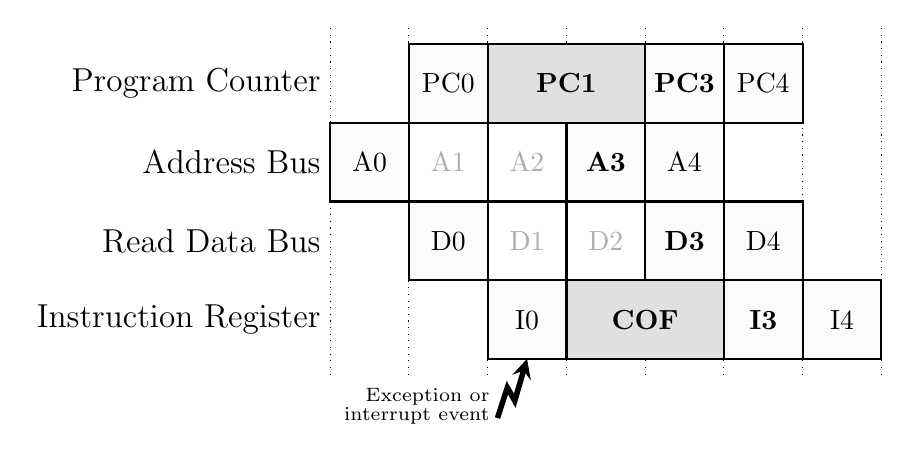
\begin{tikzpicture}

        %Lines
        \draw [dotted] (0,0.3) -- (0,4.7);
        \draw [dotted] (1,0.3) -- (1,4.7);
        \draw [dotted] (2,0.3) -- (2,4.7);
        \draw [dotted] (3,0.3) -- (3,4.7);
        \draw [dotted] (4,0.3) -- (4,4.7);
        \draw [dotted] (5,0.3) -- (5,4.7);
        \draw [dotted] (6,0.3) -- (6,4.7);
        \draw [dotted] (7,0.3) -- (7,4.7);

        %Program counter
        \node  [left] at (0,4) {\large{Program Counter}};
        \draw [thick, fill=gray!3] (1,4.5) rectangle (2,3.5);
        \node at (1.5,4)  {PC0};
        \draw [thick, fill=gray!24] (2,4.5) rectangle (4,3.5);
        \node at (3,4)  {\textbf{PC1}};
        %\draw [thick] (3,4.5) rectangle (4,3.5);
        %\node [text=gray!64] at (3.5,4)  {PC1};
        \draw [thick, fill=gray!3] (4,4.5) rectangle (5,3.5);
        \node at (4.5,4)  {\textbf{PC3}};
        \draw [thick, fill=gray!3] (5,4.5) rectangle (6,3.5);
        \node at (5.5,4)  {PC4};
        
        %Address bus
        \node [left] at (0,3) {\large{Address Bus}};
        \draw [thick, fill=gray!3] (0,3.5) rectangle (1,2.5);
        \node at (0.5,3)  {A0};1
        \draw [thick] (1,3.5) rectangle (2,2.5);
        \node [text=gray!64] at (1.5,3)  {A1};
        \draw [thick] (2,3.5) rectangle (3,2.5);
        \node [text=gray!64]  at (2.5,3)  {A2};
        \draw [thick, fill=gray!3] (3,3.5) rectangle (4,2.5);
        \node at (3.5,3)  {\textbf{A3}};
        \draw [thick, fill=gray!3] (4,3.5) rectangle (5,2.5);
        \node at (4.5,3)  {A4};

        %Read data bus
        \node [left] at (0,2) {\large{Read Data Bus}};
        \draw [thick, fill=gray!3] (1,2.5) rectangle (2,1.5);
        \node at (1.5,2)  {D0};
        \draw [thick] (2,2.5) rectangle (3,1.5);
        \node [text=gray!64] at (2.5,2)  {D1};
        \draw [thick] (3,2.5) rectangle (4,1.5);
        \node [text=gray!64] at (3.5,2)  {D2};
        \draw [thick, fill=gray!3] (4,2.5) rectangle (5,1.5);
        \node at (4.5,2)  {\textbf{D3}};
        \draw [thick, fill=gray!3] (5,2.5) rectangle (6,1.5);
        \node at (5.5,2)  {D4};

        %Instruction register
        \node [left] at (0,1) {\large{Instruction Register}};
        \draw [thick, fill=gray!3] (2,1.5) rectangle (3,0.5);
        \node at (2.5,1)  {I0};
        \draw [thick, fill=gray!24] (3,1.5) rectangle (5,0.5);
        \node at (4,1)  {\textbf{COF}};
        \draw [thick, fill=gray!3] (5,1.5) rectangle (6,0.5);
        \node at (5.5,1)  {\textbf{I3}};
        \draw [thick, fill=gray!3] (6,1.5) rectangle (7,0.5);
        \node at (6.5,1)  {I4};

        %Exception
        \draw [line width=2pt,-stealth] (2.125,-0.25) -- (2.25,0.135) -- (2.34375,-0.03125) -- (2.5,0.5);
        \node [align=right] at (1.1,-0.1) {\scriptsize{Exception or} \\[-5pt] \scriptsize{interrupt event}};

        
      \end{tikzpicture}
    }
  }
  \caption{Program flow interruted by an exception - TBD}
  \label{architecture:excyc:excpt:fig}
  \end{center}
\end{figure}


\subsection{Design Components}
\label{architecture:comp}

The N1 architecture is divided in 11 subblocks as shown in \figref{architecture:comp:fig}.

\begin{figure}[!h]
  \begin{center}
  \makebox[\textwidth][c]{
  \scalebox{1} {
      
\begin{tikzpicture}

        \node [left] at (0,0) {\large{TBD}};

      \end{tikzpicture}
    }
  }
  \caption{Block Diagram}
  \label{architecture:comp:fig}
  \end{center}
\end{figure}


\subsubsection{Flow Control Block (\texttt{fc})}
\label{architecture:fc}

The flow control block is implemented in the Verilog module \texttt{N1\_fc} (N1\_fc.v).
It manages the  \hyperref[architecture:excyc]{instruction cycles} of the N1 core.
It handles the control and resonse signals of the  \hyperref[integration:if:pbus]{program bus's} \gls{wb} interface and
it communicates with the other N1 componenents by sending requests and receiving status information.
No actual data passes through the \texttt{N1\_fc} module.
The interfaces to the N1 compunents, which are under the control of the flow control block, are explained in the following sections.

\paragraph{Control and Status Interface to the \hyperref[architecture:comp:ir]{Instruction Register}} \mbox{} \\
\label{architecture:fc:irif}

The flow control block is able to request has the following request signals to the instruction register: 
\begin{description}[style=nextline]

\item[\texttt{fc2ir\_capture}]
Capture the \hyperref[integration:if:pbus]{program bus's} read data (\texttt{pbus\_dat\_i}) in the
instruction register at the next clock edge.

\item[\texttt{fc2ir\_stash}]
Capture the \hyperref[integration:if:pbus]{program bus's} read data (\texttt{pbus\_dat\_i}) in the
stash register at the next clock edge.

\item[\texttt{fc2ir\_expend}]
The read data input of the \hyperref[integration:if:pbus]{Program Bus (\texttt{pbus\_dat\_i})}

\item[\texttt{fc2ir\_expend}]
Copy the stash regiesr's content into the instruction register at the next clock cycle.

\end{description}

The following status signala are coming from the instruction register:
%\begin{description}[style=nextline]
%\end{description}


\subsubsection{Instruction Register (\texttt{ir})}
\label{architecture:comp:ir}







%\subsubsection{Incoming Information}
%\label{architecture:ir:in}
%
%\subsubsection{Outgoing Information}
%\label{architecture:ir:out}

\subsubsection{Arithmetic Logic Unit (\texttt{alu})}
\label{architecture:comp:alu}

TBD

%\subsubsection{Incoming Information}
%\label{architecture:alu:in}

%\subsubsection{Outgoing Information}
%\label{architecture:alu:out}

\subsubsection{DSP Block (\texttt{dsp})}
\label{architecture:comp:dsp}

TBD

%\subsubsection{Incoming Information}
%\label{architecture:alu:in}

%\subsubsection{Outgoing Information}
%\label{architecture:alu:out}

\subsubsection{Exception Handler (\texttt{excpt})}
\label{architecture:comp:excpt}

TBD

%\subsubsection{Incoming Information}
%\label{architecture:alu:in}

%\subsubsection{Outgoing Information}
%\label{architecture:alu:out}

\subsubsection{Upper Stack (\texttt{us})}
\label{architecture:comp:us}

TBD

%\subsubsection{Incoming Information}
%\label{architecture:us:in}

%\subsubsection{Outgoing Information}
%\label{architecture:us:out}

\subsubsection{Intermediate Parameter Stack (\texttt{ips})}
\label{architecture:comp:ips}

TBD

%\subsubsection{Incoming Information}
%\label{architecture:ips:in}

%\subsubsection{Outgoing Information}
%\label{architecture:ips:out}

\subsubsection{Intermediate Return Stack (\texttt{irs})}
\label{architecture:comp:irs}

TBD

%\subsubsection{Incoming Information}
%\label{architecture:irs:in}

%\subsubsection{Outgoing Information}
%\label{architecture:irs:out}

\subsubsection{Lower Stack (\texttt{ls})}
\label{architecture:comp:ls}

TBD

%\subsubsection{Incoming Information}
%\label{architecture:ls:in}

%\subsubsection{Outgoing Information}
%\label{architecture:ls:out}

